\documentclass[11pt,a4paper]{article}

% ---------------------------------------------------------------------------
%  KG-Commit : First-version Knowledge Graph for commit-level bug detection
%  Build:  pdflatex KG_v1.tex   (run twice for the table of contents / refs)
% ---------------------------------------------------------------------------
\usepackage[margin=2.4cm]{geometry}
\usepackage[T1]{fontenc}
\usepackage{lmodern}
\usepackage{amsmath,amssymb}
\usepackage{booktabs}
\usepackage{longtable}
\usepackage{array}
\usepackage{xcolor}
\usepackage{enumitem}
\usepackage{caption}
\usepackage{listings}
\usepackage{graphicx}
\graphicspath{{figures/}}
\usepackage{float}
\usepackage[hidelinks]{hyperref}

\definecolor{kgblue}{HTML}{1F77B4}
\definecolor{kggreen}{HTML}{2CA02C}
\definecolor{kgred}{HTML}{D62728}
\definecolor{kgorange}{HTML}{FF7F0E}
\definecolor{kgpurple}{HTML}{9467BD}
\definecolor{codebg}{HTML}{F5F5F5}

\lstdefinestyle{cypher}{
  basicstyle=\ttfamily\small, backgroundcolor=\color{codebg},
  breaklines=true, frame=single, rulecolor=\color{gray!40},
  keywordstyle=\color{kgblue}\bfseries, columns=fullflexible,
  morekeywords={MATCH,RETURN,WHERE,WITH,MERGE,SET,CREATE,UNWIND,OPTIONAL,
                ORDER,BY,LIMIT,COUNT,DISTINCT,AS,IN,DELETE,DETACH,ON,REMOVE,collect,count}
}
\lstdefinestyle{algo}{
  basicstyle=\ttfamily\small, backgroundcolor=\color{codebg},
  breaklines=true, frame=single, rulecolor=\color{gray!40}, columns=fullflexible
}

\newcommand{\code}[1]{\texttt{#1}}
\newcommand{\node}[1]{\textcolor{kgblue}{\textbf{#1}}}
\newcommand{\edge}[1]{\textsc{#1}}

\title{\textbf{KG-Commit: A Knowledge Graph for Commit-Level Bug Detection}\\
\large First Version --- Design, Schema, and Online Growth Model}
\author{apache/groovy \;|\; ApacheJIT-labelled subset}
\date{\today}

\begin{document}
\maketitle

\begin{abstract}
This document describes the first complete version of \textbf{KG-Commit}, a
Neo4j knowledge graph built to support \emph{commit-level (just-in-time) bug
detection} on the \texttt{apache/groovy} project. The graph fuses three layers:
(i) a \emph{structural} layer of commit history (commits, developers, files,
issues); (ii) an \emph{Abstract Syntax Tree (AST)} layer that stores the actual
code structure of every source file; and (iii) a \emph{delta} layer that
connects each commit directly to the precise AST nodes it changed. The graph
grows \emph{online}: commits are ingested in chronological order, and as each
new commit arrives its modifications are modelled as a small ``delta graph''
laid on top of an evolving AST, so the whole history of every file is captured
without storing a full AST snapshot per commit. Each commit carries a
\textbf{buggy/benign} label from the ApacheJIT dataset, making the graph
directly usable for training and online evaluation of defect-prediction models.
We document every node and edge type, the exact mechanics of what happens when a
commit arrives, the correctness guarantees, the strengths and limitations of the
design for our task, and the planned next steps. We also report a first,
deliberately GPU-free inference suite: across nine classical and graph-native
methods evaluated online (prequential), an early fusion of the KG's
structural/relational signals with the classic JIT metrics lifts PR-AUC from
$0.398$ to $0.616$ ($+55\%$ relative) over the metrics-only baseline ---
evidence that the AST/delta layers carry real predictive value for commit-level
bug detection without any GNN.
\end{abstract}

\tableofcontents
\bigskip

% ===========================================================================
\section{Goal and Scope}
% ===========================================================================
The objective is a graph from which a model can \emph{infer whether a commit is
likely to introduce a bug}, using both the change itself and the surrounding
code structure. Concretely:

\begin{itemize}[nosep]
  \item \textbf{Project:} \texttt{apache/groovy} (a full local git clone).
  \item \textbf{Commit scope:} the \textbf{8{,}059 commits} that appear in the
        \textbf{ApacheJIT} dataset for groovy
        (\texttt{data/apachejit/projects/apache\_groovy.csv}), spanning
        2003--2019. These are the only commits we treat as the labelled study
        set; the local database also contains the surrounding history as
        \node{Commit} nodes, but only the ApacheJIT commits are flagged
        \code{in\_jit=true} and grown into the AST/delta layers.
  \item \textbf{Base snapshot:} commit
        \texttt{408b29851d7bbe4d343340832297e4be7e0c5578} (``BASE''), the first
        substantial Java commit, whose 120 \texttt{.java} files seed the AST
        layer.
  \item \textbf{Label:} \texttt{buggy} $\in\{$True,False$\}$ from ApacheJIT
        (1{,}614 buggy / 6{,}445 benign $\approx$ 20\% positive).
\end{itemize}

% ===========================================================================
\section{High-Level Architecture}
% ===========================================================================
The graph has three conceptual layers that share the same node space:

\begin{enumerate}[nosep]
  \item \textbf{Structural / process layer} --- the classical commit graph:
        \node{Project}, \node{Branch}, \node{Developer}, \node{Commit},
        \node{File}, \node{Issue}, and the relationships between them
        (authorship, parenthood, file changes, issue fixes).
  \item \textbf{AST layer} --- for every tracked source file, a tree of
        \node{ASTNode}s linked by \edge{AST\_CHILD}, rooted at the \node{File}
        via \edge{HAS\_AST}. Seeded from the 120 BASE files and extended as new
        files appear.
  \item \textbf{Delta layer} --- four relationship types
        (\edge{ADDS}, \edge{REMOVES}, \edge{UPDATES}, \edge{MOVES}) that connect
        a \node{Commit} \emph{directly} to the AST nodes it changed. This is the
        heart of the commit-level model.
\end{enumerate}

A small \emph{legacy} layer (\node{ASTDiff}/\node{ASTEdit}) from an earlier
experiment is still present but \textbf{deprecated} in favour of the delta layer
(\S\ref{sec:legacy}).

\paragraph{Theory.} The design is a \emph{heterogeneous information network}
(HIN): typed nodes and typed edges in one graph. This lets a single model reason
jointly over \emph{process} evidence (who changed what, when, how often) and
\emph{code-structure} evidence (the syntactic shape of the change and its
surroundings) --- the two signal sources the defect-prediction literature treats
separately. Anchoring commit changes to \emph{shared, persistent} AST nodes
(rather than to per-commit summary blobs) is what enables relational and
neighbourhood reasoning across the whole history.

\paragraph{Practice.} The structural/process layer is produced in \texttt{kg\_commit/knowledge}, (driven from the ApacheJIT CSV
and the local git clone). The AST layer is seeded once
(\texttt{build\_file\_ast\_graphs.py} $+$ \texttt{ingest\_base\_kg\_and\_ast.py}),
positions are stamped (\texttt{add\_positions\_to\_astnodes.py}), labels are
applied (\texttt{apply\_commit\_labels.py}), and the delta layer is grown by the
online engine (\texttt{build\_online\_kg.py}, using
\texttt{online\_ast\_diff.py}). Everything is stored in one Neo4j database.

% ===========================================================================
\section{Node Types}
% ===========================================================================
Table~\ref{tab:nodes} lists every node label, its meaning, and its key
properties.

\begin{longtable}{@{}p{2.4cm}p{4.4cm}p{7.6cm}@{}}
\caption{Node types.}\label{tab:nodes}\\
\toprule
\textbf{Label} & \textbf{Meaning} & \textbf{Key properties}\\
\midrule
\endfirsthead
\toprule
\textbf{Label} & \textbf{Meaning} & \textbf{Key properties}\\
\midrule
\endhead
\node{Project} & The repository. & \code{id} (e.g.\ \texttt{apache/groovy}).\\
\addlinespace
\node{Branch} & A git branch. & \code{id}.\\
\addlinespace
\node{Developer} & A commit author. & \code{id} (name/email).\\
\addlinespace
\node{Commit} & A single commit. & \code{id} (40-char SHA), \code{message},
  \code{committed\_at}, \code{author\_ts} (UNIX seconds = online order),
  \code{in\_jit}, \code{buggy}, \code{is\_fix}, \code{jit\_year}, and the
  ApacheJIT change metrics \code{la}, \code{ld}, \code{nf}, \code{nd},
  \code{ns}, \code{ent}, \code{ndev}, \code{age}, \code{nuc}, \code{aexp},
  \code{arexp}, \code{asexp}.\\
\addlinespace
\node{File} & A repository-relative file path. & \code{id} (path).\\
\addlinespace
\node{Issue} & A referenced issue (e.g.\ \texttt{GROOVY-20}). & \code{id}.\\
\addlinespace
\node{ASTNode} & One node of a file's AST (declaration, statement, expression,
  literal, or identifier leaf). & \code{id} =
  \texttt{\{file\}::A\{i\}} for original nodes or
  \texttt{\{file\}::D\{sha8\}:\{i\}} for nodes inserted by a commit;
  \code{file}, \code{ast\_type} (javalang type), \code{group}
  (\texttt{declaration}/\texttt{statement}/\texttt{expression}/\texttt{literal}/\texttt{leaf}),
  \code{value}, \code{is\_leaf}, \code{depth}, \code{pos\_line},
  \code{pos\_col}, and on evolving nodes \code{alive} (false once removed),
  \code{removed\_by}, \code{is\_delta} (true if inserted by a commit).\\
\addlinespace
\node{ASTDiff} \emph{(legacy)} & Per-(commit,file) diff summary. &
  \code{id}, \code{commit\_id}, \code{file}, \code{n\_insert/delete/update/move},
  \code{total}.\\
\addlinespace
\node{ASTEdit} \emph{(legacy)} & A single GumTree edit action. &
  \code{action}, \code{node\_type}, \code{node\_label}, \code{new\_label},
  \code{parent\_type}, \code{position}.\\
\bottomrule
\end{longtable}

\paragraph{AST node identity.} Node ids are \emph{deterministic}: the same
source file always yields the same \texttt{\{file\}::A\{i\}} ids, where $i$ is a
pre-order DFS counter from the AST builder. This determinism is what lets us
thread node identity across versions of a file (\S\ref{sec:online}).

% ===========================================================================
\section{Edge Types}
% ===========================================================================
Table~\ref{tab:edges} groups the relationships by layer.

\begin{longtable}{@{}p{3.0cm}p{3.0cm}p{8.4cm}@{}}
\caption{Relationship types.}\label{tab:edges}\\
\toprule
\textbf{Type} & \textbf{From $\rightarrow$ To} & \textbf{Meaning / properties}\\
\midrule
\endfirsthead
\toprule
\textbf{Type} & \textbf{From $\rightarrow$ To} & \textbf{Meaning / properties}\\
\midrule
\endhead
\multicolumn{3}{@{}l}{\textit{Structural / process layer}}\\
\midrule
\edge{BELONGS\_TO} & Commit $\rightarrow$ Project & Commit is part of the project.\\
\edge{INSIDE\_BRANCH} & Branch $\rightarrow$ Commit & Commit is on the branch.\\
\edge{PARENT\_OF} & Commit $\rightarrow$ Commit & Git parent relation (history spine).\\
\edge{AUTHORED\_BY} & Commit $\rightarrow$ Developer & Authorship.\\
\edge{FIXES\_ISSUE} & Commit $\rightarrow$ Issue & Commit message references/fixes an issue.\\
\midrule
\multicolumn{3}{@{}l}{\textit{File-change layer}}\\
\midrule
\edge{ADDED} & Commit $\rightarrow$ File & File added by the commit.\\
\edge{MODIFIED} & Commit $\rightarrow$ File & File modified by the commit.\\
\edge{DELETED} & Commit $\rightarrow$ File & File deleted by the commit.\\
\edge{RENAMED\_FROM} and \edge{RENAMED\_TO} & Commit $\rightarrow$ File & File rename endpoints.\\
\midrule
\multicolumn{3}{@{}l}{\textit{AST layer}}\\
\midrule
\edge{HAS\_AST} & File $\rightarrow$ ASTNode & Links a file to its AST root node.\\
\edge{AST\_CHILD} & ASTNode $\rightarrow$ ASTNode & Parent-to-child tree edge;
  property \code{pos} = child ordinal.\\
\midrule
\multicolumn{3}{@{}l}{\textit{Delta layer (the commit-level model)}}\\
\midrule
\textcolor{kggreen}{\edge{ADDS}} & Commit $\rightarrow$ ASTNode & The commit
  \emph{inserted} this node (node has \code{is\_delta=true}); the node is also
  wired into the tree via a new \edge{AST\_CHILD} edge to its parent.\\
\textcolor{kgred}{\edge{REMOVES}} & Commit $\rightarrow$ ASTNode & The commit
  \emph{deleted} this node; the node is kept but marked \code{alive=false},
  \code{removed\_by}=commit (history preserved).\\
\textcolor{kgorange}{\edge{UPDATES}} & Commit $\rightarrow$ ASTNode & The commit
  changed the node's value; properties \code{old\_value}, \code{new\_value}.\\
\textcolor{kgpurple}{\edge{MOVES}} & Commit $\rightarrow$ ASTNode & The commit
  relocated the node; property \code{new\_parent\_type}.\\
\midrule
\multicolumn{3}{@{}l}{\textit{Legacy layer (deprecated)}}\\
\midrule
\edge{HAS\_AST\_DIFF} & Commit $\rightarrow$ ASTDiff & old per-file diff summary.\\
\edge{EDIT} & ASTDiff $\rightarrow$ ASTEdit & one edit of the diff.\\
\edge{DIFFED\_AT} & File $\rightarrow$ ASTDiff & file the diff applies to.\\
\bottomrule
\end{longtable}

% ===========================================================================
\section{The Base Graph}
% ===========================================================================
The AST layer is seeded at the BASE commit. Each of the 120 \texttt{.java} files
is parsed with the \texttt{javalang} library and converted to a graph by a
pre-order traversal that assigns every node a stable id
\texttt{\{file\}::A\{i\}}. Two kinds of nodes are produced:

\begin{itemize}[nosep]
  \item \textbf{Structured nodes} ($\approx$36\%): real \texttt{javalang.tree}
        nodes (classes, methods, fields, statements, expressions, literals),
        carrying a source position (\code{pos\_line}, \code{pos\_col}).
  \item \textbf{Identifier leaves} ($\approx$64\%): raw string children
        (identifier and operator tokens) that javalang attaches to a node; these
        have no source position (\code{pos\_line}=$-1$).
\end{itemize}

Each file is attached as
\edge{File} $\xrightarrow{\text{HAS\_AST}}$ \edge{root}
$\xrightarrow{\text{AST\_CHILD}^{*}}$ \edge{descendants}.
At BASE this is 120 files and $\approx$46k AST nodes. This is the
``previous structure'' onto which all later commit deltas are laid.

\paragraph{Theory.} An AST abstracts away surface formatting and records the
grammatical structure of code; making it an explicit subgraph (rather than a
flat token sequence) lets downstream models exploit parent/child and
type-of-node relations. Choosing one consistent parser (javalang) for the whole
graph is what makes node identities comparable across file versions
(\S\ref{sec:identity}).

\paragraph{Implementation.} \texttt{build\_file\_ast\_graphs.py} parses each
BASE file in a killable subprocess (javalang can hang on pathological input) and
emits a \texttt{networkx} graph whose node ids are the deterministic
\texttt{\{file\}::A\{i\}} counters; \texttt{ingest\_base\_kg\_and\_ast.py}
\texttt{MERGE}s these into Neo4j under each \node{File};
\texttt{add\_positions\_to\_astnodes.py} re-runs the identical traversal to stamp
\code{pos\_line}/\code{pos\_col} on every node.

% ===========================================================================
\section{Online Growth: What Happens When a Commit Arrives}\label{sec:online}
% ===========================================================================
\paragraph{Theory.} The problem of describing how one tree becomes another is
\emph{tree differencing} / tree edit distance: find a minimal-cost set of
insert/delete/update/move operations mapping a ``before'' tree to an ``after''
tree. Equivalently, one seeks a \emph{matching} between the two node sets;
unmatched before-nodes are deletions, unmatched after-nodes are insertions, and
matched nodes whose label differs are updates. We compute this matching and
record each operation as a typed edge from the commit to the affected AST node.
Modelling change as a delta (operations) rather than as two stored snapshots is
both information-preserving and asymptotically smaller: storage grows with the
\emph{amount of change}, not with history length $\times$ file size.

\paragraph{Practice.} Commits are processed in \textbf{chronological order}
(\code{author\_ts}). The engine (\texttt{build\_online\_kg.py}) maintains, per
tracked file, the \emph{current} state of its AST in the graph. When commit $C$
arrives, it computes the set of changed \texttt{.java} files (\code{git diff} of
$C$ against its first parent) and, for each file, takes one of four actions.

\begin{lstlisting}[style=algo,caption={Per-commit processing.}]
for each commit C in stream order (by author_ts):
    for each changed .java file F of C (status A / M / D):

        if status == DELETED:
            mark every alive ASTNode of F as alive=false, removed_by=C
            add (C)-[:REMOVES]->(node) for each
            stop tracking F

        elif status == ADDED  OR  F has no AST yet (lazy bootstrap):
            build the FULL AST of F (from C for ADDED, or from C^1 if the
                file already existed but was never tracked)
            attach File-[:HAS_AST]->root and the AST_CHILD tree
            if ADDED: add (C)-[:ADDS]->(node) for every node of the new file
            # an untracked-but-modified file is bootstrapped at C^1 and then
            # falls through to the MODIFIED case below

        if status == MODIFIED (file is tracked):
            diff the file's stored state  ->  its content at C   (see 7.1)
            apply the resulting delta to the graph (see 7.2)
    label of C (buggy/benign) is already on the Commit node
    checkpoint progress (resumable)
\end{lstlisting}

\subsection{Diffing a modified file}
The modify path uses a \textbf{javalang-native tree differ}
(\texttt{online\_ast\_diff.py}). Both the ``before'' state (the file's stored
content) and the ``after'' state (its content at $C$) are parsed with the
\emph{same} builder used for the graph, so their node ids are directly
comparable. Matching proceeds in three stages:

\begin{enumerate}[nosep]
  \item \textbf{Subtree-hash, bottom-up:} every subtree is hashed by
        (type, value, children hashes); identical subtrees in before/after are
        matched greedily, preferring equal source positions. This matches the
        large \emph{unchanged} majority of the file exactly.
  \item \textbf{Parent propagation, top-down:} if two matched nodes have
        unmatched parents of the same type, the parents are matched. This covers
        changed-but-aligned ancestors.
  \item \textbf{Positional fallback:} any remaining node is matched by
        (type, line, col).
\end{enumerate}

The differ outputs four sets: \emph{matched} (with a value-changed flag),
\emph{deleted}, \emph{inserted}, and \emph{moved}.

\subsection{Applying the delta and evolving the structure}
The delta is written to Neo4j and the stored AST is evolved so that the next
commit diffs against the correct state:

\begin{itemize}[nosep]
  \item \textbf{matched} nodes keep their graph id; their position is re-stamped
        to the new source location; if the value changed, an \edge{UPDATES} edge
        is added and the node's \code{value} is updated.
  \item \textbf{deleted} nodes are marked \code{alive=false}, \code{removed\_by}=$C$,
        and a \edge{REMOVES} edge is added (the node is \emph{kept} for history).
  \item \textbf{inserted} nodes are created (\code{is\_delta=true}), wired into
        the tree with a new \edge{AST\_CHILD} edge to their (existing or newly
        inserted) parent, and an \edge{ADDS} edge is added.
  \item \textbf{moved} nodes get a \edge{MOVES} edge recording the new parent type.
\end{itemize}

\subsection{Node identity across versions}\label{sec:identity}
Correctly carrying a node's identity from one version of a file to the next is
the crux of the model. We thread identity with a per-file map
\texttt{\{parse-local-id $\rightarrow$ graph-node-id\}}. Because the same source
deterministically yields the same parse-local ids, the ``after'' map of commit
$C$ is exactly the ``before'' map of the next commit that touches the file. Base
files start from the identity map (graph id $=$ parse id).

\paragraph{Why not GumTree or position matching?} An earlier version matched
GumTree's diff actions back to graph nodes by source \emph{position}. This
\emph{drifted}: GumTree parses a different tree (JavaParser/JDT) than our
javalang graph, and $\approx$32\% of AST nodes share a \texttt{(line,col)} with
another node, so re-stamping mis-assigned them. Measured against ground truth,
the position-based evolution achieved only \textbf{recall 0.41}. The
javalang-native differ with deterministic identity achieves
\textbf{precision $=$ recall $=$ 1.000} on the validation window: the graph's
``alive'' AST of every evolved file is byte-for-byte the AST of the real file at
its current state.

\subsection{Why this is space- and time-efficient}
Only \emph{one} evolving AST is kept per file, plus the delta edges; we never
store a separate full AST per commit. A commit that changes three lines adds a
handful of delta edges, not a fresh copy of the file's tree. Removed nodes are
retained (flagged) so the complete change history is queryable while the live
tree always reflects the current code.

% ===========================================================================
\section{Labels for Bug Detection}
% ===========================================================================
Every ApacheJIT commit is annotated (\texttt{apply\_commit\_labels.py}) with
\code{buggy}, \code{is\_fix}, \code{author\_ts} (online order), \code{jit\_year},
and the standard JIT change metrics. The class balance is $\approx$20\% buggy.
A quick sanity check confirms signal: buggy commits are on average much larger
(mean lines added $\approx$196 vs.\ $\approx$70 for benign) and more scattered
(mean change entropy $\approx$1.26 vs.\ $\approx$0.73).

For \emph{online} evaluation, the \code{author\_ts} ordering lets one reproduce
the exact information available when each commit ``arrives'': all earlier
commits' labels are known, the one under test is not.

% ===========================================================================
\section{Statistics (finalized full build)}
% ===========================================================================
Final sizes of the assembled graph after the complete online build over all
8{,}059 labelled commits.

\begin{center}
\begin{tabular}{@{}lr@{}}
\toprule
\textbf{Element} & \textbf{Count}\\
\midrule
\node{Commit} (total in DB) & 16{,}887\\
\quad of which ApacheJIT-labelled (\code{in\_jit}) & 8{,}059\\
\quad buggy / benign & 1{,}614 / 6{,}445\\
\quad carrying AST deltas & 7{,}521\\
\node{ASTNode} & 3{,}635{,}438\\
\quad inserted by commits (\code{is\_delta}) & 1{,}249{,}170\\
\quad removed (\code{alive=false}, kept as history) & 807{,}120\\
\quad alive / untouched-base (\code{alive=NULL}) & 2{,}805{,}375 / 22{,}943\\
\quad positioned (have \code{pos\_line}$>$0) & 1{,}233{,}500\\
\node{File} & 5{,}655\\
\quad with an AST (\edge{HAS\_AST}) & 3{,}006\\
\quad born during the stream (post-BASE) & 1{,}611\\
\node{Issue} / \node{Developer} & 4{,}877 / 319\\
\midrule
\edge{AST\_CHILD} & 3{,}652{,}425\\
\edge{ADDS} & 2{,}337{,}767\\
\edge{REMOVES} & 818{,}063\\
\edge{MOVES} & 147{,}330\\
\edge{UPDATES} & 13{,}316\\
\edge{MODIFIED} / \edge{ADDED} / \edge{DELETED} & 35{,}252 / 3{,}466 / 1{,}602\\
\edge{PARENT\_OF} / \edge{AUTHORED\_BY} & 13{,}122 / 13{,}121\\
\edge{FIXES\_ISSUE} & 6{,}404\\
\bottomrule
\end{tabular}
\end{center}

On disk the graph store is $\approx$3.3\,GB; with transaction logs the working
footprint is $\approx$5.6\,GB (budget $\approx$10\,GB for headroom).

\paragraph{Bug signal.} Buggy commits make structurally much larger AST changes
than benign ones: on average $\approx$860 delta edges per buggy commit versus
$\approx$299 per benign commit (and $\approx$196 vs.\ $\approx$70 lines added).
This separation is the basic reason the graph is useful for the task.
Figure~\ref{fig:signal} shows both this size separation and the strong
\emph{temporal drift} of the bug rate across 2003--2019 --- the latter being why
a time-aware online protocol (\S\ref{sec:inference}) is essential.

\begin{figure}[H]\centering
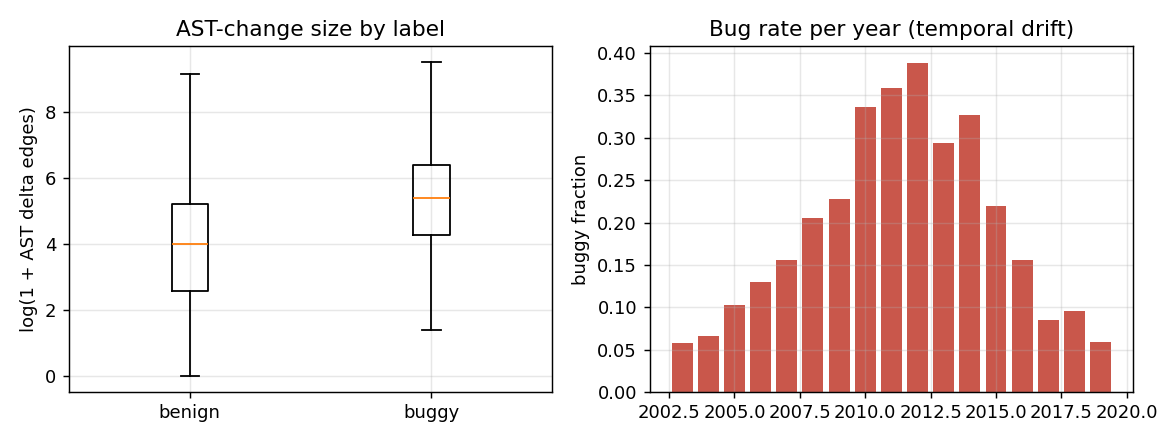
\includegraphics[width=.92\linewidth]{bug_signal.png}
\caption{Left: AST-change size (log delta edges) for benign vs.\ buggy commits.
Right: yearly bug rate, showing pronounced concept drift.}\label{fig:signal}
\end{figure}

% ===========================================================================
\section{Audit and Data Quality of the Finalized KG}\label{sec:audit}
% ===========================================================================
We audited the complete graph (see \texttt{neo4j\_queries.txt}, Section~13). The
schema is clean and coverage is high; the few gaps are small and explainable.

\begin{center}
\begin{tabular}{@{}p{9.2cm}rl@{}}
\toprule
\textbf{Check} & \textbf{Result} & \textbf{Verdict}\\
\midrule
in\_jit commits carrying an AST delta & 7{,}521 / 8{,}059 & expected\\
in\_jit commits with \emph{no} AST delta & 538 & explainable$^{a}$\\
\texttt{.java} files modified by a labelled commit but never parsed & 5 & gap$^{b}$\\
Files with $>$1 AST root (duplicate-attach bug) & 0 & clean\\
No-op \edge{UPDATES} (\code{old\_value}=\code{new\_value}) & 4 & negligible\\
Removed nodes lacking a \edge{REMOVES} edge & 0 & clean\\
\node{File} nodes total & 5{,}655 & ---\\
\quad \texttt{.java} with an AST & 3{,}006 & expected\\
\quad \texttt{.java} \emph{without} an AST & 2{,}628 & out-of-scope$^{c}$\\
\quad non-\texttt{.java} (\texttt{.groovy}, \texttt{temp/}) & 21 & expected\\
\bottomrule
\end{tabular}
\end{center}

\footnotesize
$^{a}$ These commits changed only non-Java files (build scripts, resources,
docs) or made import-only/whitespace edits that produce no AST-structural change.
$^{b}$ Six Java files fail both the JavaParser and JDT parsers (unusual legacy
syntax in the old \texttt{lexer/}/\texttt{parser/} sources); they have
commit/file nodes but no AST subtree. $^{c}$ \textbf{Important scoping fact:}
\node{File} nodes are created from the \emph{full} ingested commit history, but
the AST/delta layer is grown only for files touched by the 8{,}059 labelled
(\code{in\_jit}) commits. Of the 2{,}628 \texttt{.java} files without an AST,
only \textbf{6} were ever touched by a labelled commit (the parser-failure gaps
above); the other $\approx$2{,}622 were touched \emph{only by non-labelled
commits} and are therefore intentionally outside the modelled scope. This does
not affect inference, which uses only the labelled commits and their deltas.
\normalsize

% ===========================================================================
\section{Strengths and Limitations for Commit-Level Bug Detection}
% ===========================================================================
\subsection*{Strengths}
\begin{itemize}[nosep]
  \item \textbf{Change in context.} A commit is linked to the \emph{exact} AST
        nodes it touched \emph{and} to the surrounding code structure, so a GNN
        can reason over both the change and its neighbourhood --- richer than
        hand-crafted JIT metrics alone.
  \item \textbf{Lossless, incremental history.} Every file's evolution is
        captured exactly (recall 1.0) with only deltas stored; removed nodes are
        retained, so any past state is reconstructable.
  \item \textbf{Multi-modal.} Process signals (author, churn, issue links,
        history spine) and code-structure signals live in one graph and can be
        combined.
  \item \textbf{Online-ready.} Chronological \code{author\_ts} ordering and the
        arrival model directly support time-aware train/test splits and
        streaming evaluation, avoiding look-ahead leakage.
  \item \textbf{Labels built in.} ApacheJIT buggy/benign plus JIT metrics are on
        every commit node.
\end{itemize}

\subsection*{Limitations}
\begin{itemize}[nosep]
  \item \textbf{Filtered commit set.} Only the 8{,}059 ApacheJIT commits are
        grown; deltas between two consecutive labelled commits that touch the
        same file therefore bundle any intervening \emph{unlabelled} commits.
        The change attributed to a commit is ``since the last labelled touch,''
        which may slightly differ from its raw git parent diff.
  \item \textbf{Java-only.} Non-\texttt{.java} files (build scripts, resources)
        are not modelled at the AST level.
  \item \textbf{Coarse value handling.} \edge{UPDATES} captures a node's value
        change but not deep semantic equivalence; renames look like updates.
  \item \textbf{Identifier leaves lack positions} and are matched structurally
        only; very large refactors can stress the heuristic matcher (still
        consistent, but matches may be sub-optimal versus a full GumTree).
  \item \textbf{Label semantics.} ApacheJIT labels are derived (SZZ-style); they
        carry the usual noise of automatically mined defect labels.
  \item \textbf{Operational.} The build is long (hours) and, in this version,
        used a large resumable checkpoint; node identity should move onto the
        graph to keep checkpoints small (see next steps).
\end{itemize}

% ===========================================================================
\section{Downstream Inference}\label{sec:inference}
% ===========================================================================
This section reports the first inference suite built on top of the KG. Because
the target hardware has \emph{no GPU}, every method is deliberately light and
\textbf{GNN-free}; the goal is both a usable defect predictor and a set of strong
baselines a future GNN must beat. All code lives in \texttt{inference/}.

\subsection{Problem framing (theory)}
Just-in-time (JIT) defect prediction is a \emph{streaming binary
classification} problem: each commit $C$ is a point with label
$y_C\in\{\text{buggy},\text{benign}\}$, and predictions must be made
\emph{at commit time} using only information available then. Formally, for a
commit arriving at time $t_C$ (\code{author\_ts}), a model may use any data from
commits with $t<t_C$ but nothing from the future. This rules out a random
train/test split (which leaks future information) and demands a
\emph{prequential} (predict-then-update) protocol. The positive class is rare
($\approx$20\%), so threshold-free ranking metrics --- ROC-AUC and especially
PR-AUC (area under precision--recall) --- are the primary measures; F1/MCC at a
$0.5$ threshold are secondary.

\subsection{Features from the KG (theory + implementation)}
Three feature families are read out of the graph
(\texttt{extract\_features.py}, \texttt{run\_all.py}):
\begin{description}[nosep,leftmargin=1.4em]
  \item[Process metrics.] The 12 ApacheJIT change metrics already on each
        \node{Commit} (size \code{la}/\code{ld}, dispersion \code{nf}/\code{ent},
        history/experience \code{age}/\code{ndev}/\code{aexp}\ldots). \emph{Theory:}
        larger, more scattered, less-familiar changes are historically more
        defect-prone. \emph{Practice:} read directly as a $12$-dim vector.
  \item[Delta-graph features.] Per commit, counts and node-type/group histogram
        of its \edge{ADDS}/\edge{REMOVES}/\edge{UPDATES}/\edge{MOVES} edges, plus
        ``AST-change tokens'' \code{\{edge\}:\{ast\_type\}}
        (e.g.\ \code{ADDS:MethodInvocation}). \emph{Theory:} the \emph{shape} of a
        structural change carries risk information beyond its size. \emph{Practice:}
        one Cypher aggregation over the delta layer.
  \item[Topology.] The heterogeneous neighbourhood of a commit (its files,
        developer, issues, changed AST types) used by the propagation and
        embedding methods below.
\end{description}

\subsection{Methods (theory + implementation)}
\begin{description}[nosep,leftmargin=1.4em]
  \item[JIT-metrics baseline.] Logistic regression / random forest / gradient
        boosting on the 12 metrics --- the standard JIT predictor
        (\texttt{train\_eval.py}).
  \item[wvRN / relational priors.] \emph{Weighted-vote relational neighbour}: a
        commit's score is the historical bug-rate of the files and developer it
        touches, computed from the past only (\texttt{online\_infer.py}). Classic
        collective-classification baseline; very cheap, leakage-free.
  \item[Structural TF-IDF.] Treat each commit as a ``document'' of its AST-change
        tokens; TF-IDF $+$ linear model (\texttt{advanced\_infer.py}). Learns
        \emph{which kinds} of edits predict bugs.
  \item[Personalized PageRank (PPR).] Random-walk-with-restart label propagation
        over the heterogeneous KG, seeded from past buggy vs.\ benign commits;
        a commit is scored by relative proximity to each class
        (\texttt{advanced\_infer.py}). The textbook non-GNN graph inference.
  \item[KG embeddings.] Shallow, CPU-only graph embeddings feeding a linear
        classifier (\texttt{kge\_infer.py}): \emph{Truncated-SVD/LSA} of the
        commit--hub matrix; \emph{node2vec/DeepWalk} random-walk skip-gram
        (gensim); and \emph{TransE}/\emph{DistMult} knowledge-graph embeddings
        (PyKEEN, trained without the costly link-prediction evaluation).
  \item[Fusion.] Early fusion (one regularised linear model) over JIT metrics
        $+$ structural TF-IDF $+$ relational priors $+$ PPR score
        (\texttt{run\_all.py}).
\end{description}

\subsection{Evaluation protocols}
Two protocols are run for every method. \textbf{Offline} uses a single
time-ordered $70/30$ split (train on the older $70\%$). \textbf{Online}
(prequential) warms up on the first $40\%$ then streams the rest in blocks,
predicting each block from a model trained only on strictly earlier commits
(expanding window). Online is the protocol that matches deployment; offline is a
convenient sanity check. Leakage controls: scalers/vectorisers/embedding
classifiers are fit on past data only, and the PPR score is computed with
chronological folds so a commit is never among its own seeds.

\subsection{Results}
Tables~\ref{tab:off} and~\ref{tab:on} give every method in both protocols
(consolidated by \texttt{run\_all.py}; the executed notebook
\texttt{experiments/notebooks/inference\_results.ipynb} renders the same numbers
as bar charts, ROC/PR curves and a heatmap). Random PR-AUC equals the positive
rate: $0.163$ offline, $0.245$ online.

\begin{table}[h]\centering\small
\caption{Offline (time-ordered $70/30$ split).}\label{tab:off}
\begin{tabular}{@{}lrrrr@{}}
\toprule
\textbf{Method} & \textbf{ROC-AUC} & \textbf{PR-AUC} & \textbf{F1} & \textbf{MCC}\\
\midrule
JIT-metrics (baseline) & 0.739 & 0.355 & 0.411 & 0.280\\
wvRN / priors          & 0.787 & 0.408 & 0.081 & 0.127\\
Structural TF-IDF      & 0.731 & 0.404 & 0.395 & 0.256\\
PPR propagation        & 0.687 & 0.273 & 0.338 & 0.170\\
KGE Truncated-SVD      & 0.691 & 0.306 & 0.382 & 0.234\\
node2vec               & 0.749 & 0.405 & 0.399 & 0.264\\
TransE                 & 0.726 & 0.360 & 0.386 & 0.247\\
DistMult               & 0.768 & 0.438 & 0.437 & 0.317\\
\textbf{Fusion}        & \textbf{0.820} & \textbf{0.542} & \textbf{0.477} & \textbf{0.376}\\
\bottomrule
\end{tabular}
\end{table}

\begin{table}[h]\centering\small
\caption{Online (prequential, expanding window) --- the deployment protocol.}\label{tab:on}
\begin{tabular}{@{}lrrrr@{}}
\toprule
\textbf{Method} & \textbf{ROC-AUC} & \textbf{PR-AUC} & \textbf{F1} & \textbf{MCC}\\
\midrule
JIT-metrics (baseline) & 0.679 & 0.398 & 0.453 & 0.218\\
wvRN / priors          & 0.733 & 0.460 & 0.067 & 0.115\\
Structural TF-IDF      & 0.750 & 0.489 & 0.519 & 0.333\\
PPR propagation        & 0.681 & 0.351 & 0.471 & 0.245\\
KGE Truncated-SVD      & 0.703 & 0.442 & 0.460 & 0.279\\
node2vec               & 0.740 & 0.471 & 0.506 & 0.306\\
TransE                 & 0.730 & 0.469 & 0.497 & 0.292\\
DistMult               & 0.757 & 0.487 & 0.529 & 0.343\\
\textbf{Fusion}        & \textbf{0.827} & \textbf{0.616} & \textbf{0.555} & \textbf{0.397}\\
\bottomrule
\end{tabular}
\end{table}

\begin{figure}[H]\centering
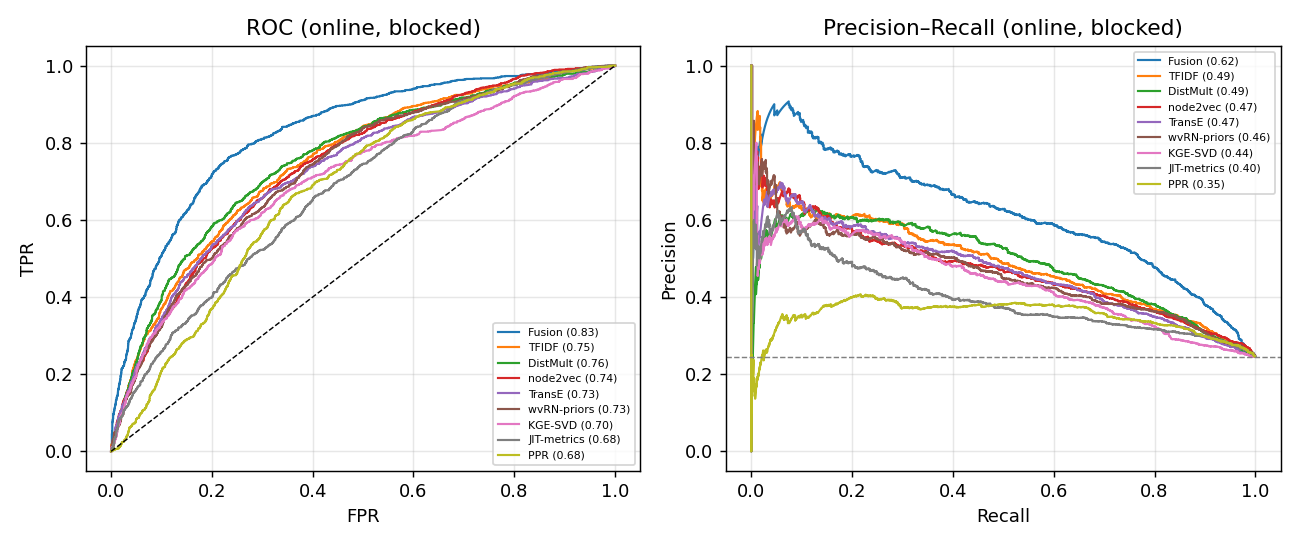
\includegraphics[width=\linewidth]{online_curves.png}
\caption{Online (blocked) ROC and precision--recall curves. Fusion (top legend
entry) dominates across the whole operating range; every KG-native method sits
above the JIT-metrics baseline on PR.}\label{fig:curves}
\end{figure}

\subsection{Interpretation}
\begin{itemize}[nosep]
  \item \textbf{Fusion is best by a wide margin}, and the gap is largest in the
        deployment-realistic online setting: PR-AUC $0.398\!\rightarrow\!0.616$
        over the JIT baseline ($+55\%$ relative), ROC $0.679\!\rightarrow\!0.827$,
        MCC $0.218\!\rightarrow\!0.397$. \emph{The KG's AST/delta and relational
        signals add real, complementary predictive value} on top of the classic
        metrics --- the central justification for the graph.
  \item \textbf{Every KG-native signal beats the metrics baseline on PR-AUC
        online.} The strongest \emph{single} signals are structural TF-IDF
        ($0.489$) and the DistMult embedding ($0.487$): \emph{what kind} of AST
        change a commit makes, and \emph{where} the commit sits in the
        heterogeneous graph, are both individually informative.
  \item \textbf{Embeddings.} DistMult (bilinear) $>$ node2vec $\approx$ TransE
        $>$ Truncated-SVD, consistent with bilinear scoring capturing the
        commit--type--file relations better than a purely translational or
        linear-spectral model.
  \item \textbf{PPR alone is weak} ($0.351$): file/developer hubs connect buggy
        and benign commits indiscriminately, so raw proximity is noisy --- yet it
        still helps inside the fusion as one signal among many.
  \item \textbf{Online $>$ offline} for most methods because the
        expanding-window retraining \emph{adapts to concept drift} (the bug rate
        rises then falls across 2003--2019); this is exactly why the online
        protocol matters for JIT.
  \item \textbf{Caveat.} wvRN's near-zero F1 reflects an uncalibrated raw-rate
        score (its ranking, ROC/PR, is strong); a threshold/calibration step
        fixes the hard-decision metric.
\end{itemize}

\subsection{Controlled comparison to the project baselines}\label{sec:cmp}
The within-project baselines in \texttt{baselines/} (notebook
\texttt{WithinProj\_baselines.ipynb}) evaluate on a single \emph{chronological}
split per project --- sort by \code{author\_date}, train on the first $70\%$,
test on the \emph{last} $15\%$ (the middle $15\%$ validation block is unused) ---
and report ROC-AUC and buggy-class F1. To compare fairly we re-ran our own
features through that \emph{exact} split and test set
(\texttt{inference/compare\_baselines.py}); every ``Ours'' row uses a
\emph{balanced logistic regression}, identical to the baseline classifier, so any
difference comes from the \emph{features}, not the learner. As a sanity check our
JIT-metrics model reproduces the baseline logistic regression \emph{exactly}
(ROC $0.698$, F1 $0.232$), confirming the protocols are aligned.

\paragraph{Caution on the window.} This split's test set is the last $15\%$ of
the timeline (2018--2019), where the bug rate is only $\approx$7.5\% --- a much
lower and harder regime than the windows of
Tables~\ref{tab:off}--\ref{tab:on} (bug rate $0.16$/$0.25$). Absolute scores are
therefore lower here and are \emph{not} directly comparable to those tables;
within Table~\ref{tab:base} everything is on the same footing.

\begin{table}[h]\centering\small
\caption{Controlled comparison on the baselines' chronological split (train first
$70\%$, test last $15\%$; test bug rate $\approx0.075$). ``Ours'' rows use a
balanced logistic regression on the named KG features.}\label{tab:base}
\begin{tabular}{@{}lrr@{}}
\toprule
\textbf{Method} & \textbf{ROC-AUC} & \textbf{F1}\\
\midrule
\multicolumn{3}{@{}l}{\textit{Published baselines (\texttt{baselines/results})}}\\
Naive: random / all-buggy & 0.500 & 0.09\,/\,0.13\\
JIT metrics --- Logistic Regression & 0.698 & 0.232\\
JIT metrics --- Random Forest (tuned) & 0.729 & 0.336\\
JIT metrics --- XGBoost (tuned) & 0.755 & 0.267\\
Text TF-IDF-768D --- Random Forest & \textbf{0.813} & 0.321\\
\midrule
\multicolumn{3}{@{}l}{\textit{Ours --- same split, balanced LR on KG features}}\\
JIT-metrics (reproduces baseline LR) & 0.698 & 0.232\\
Structural TF-IDF (AST tokens) & 0.637 & 0.217\\
PPR propagation & 0.667 & 0.166\\
KG embeddings (SVD / node2vec / TransE / DistMult) & 0.61--0.62 & $\sim$0.21\\
wvRN / relational priors & 0.743 & 0.000\\
\textbf{Fusion (JIT $+$ TF-IDF $+$ priors $+$ PPR)} & \textbf{0.732} & \textbf{0.236}\\
\bottomrule
\end{tabular}
\end{table}

\paragraph{Honest reading.}
\begin{itemize}[nosep]
  \item Our \textbf{Fusion (ROC $0.732$)} is \emph{competitive with the tuned
        traditional-metric baselines} (RF-tuned $0.729$, just under
        XGBoost-tuned $0.755$) and well above plain JIT-LR ($0.698$), but it does
        \textbf{not} beat the strongest baseline --- a \emph{text} TF-IDF-768D
        model ($0.813$).
  \item Our individual KG-native methods \emph{underperform} on this hard,
        low-bug tail window (ROC $0.61$--$0.74$) --- noticeably weaker than they
        look on the easier windows of Tables~\ref{tab:off}--\ref{tab:on}.
  \item The decisive gap is that the best baseline uses \textbf{commit-message /
        code text} (a $768$-dim embedding), a signal our KG inference does
        \emph{not} use at all. Code-structure and process signals alone are
        competitive with traditional metrics but not with strong text features on
        this split.
\end{itemize}
This \emph{corrects} an earlier, non-controlled comparison (which compared
different test windows and overstated our advantage). The implication is item~1
of \S\ref{sec:next}: add commit-text features to the fusion and/or move to a GNN
that exploits the AST neighbourhood the tabular methods flatten away.

\subsection{Fully-online (prequential) evaluation and operating-point F1}\label{sec:onlinejit}
The strictest realisation of the JIT protocol processes commits \emph{one at a
time}: as each commit arrives we (1)~\textbf{predict} it from the KG/history
known so far, (2)~\textbf{evaluate} by revealing its label and updating running
metrics, (3)~\textbf{grow} the KG state (its relational/graph evidence is added),
and (4)~\textbf{learn} (incremental \code{partial\_fit} for linear models,
periodic expanding-window retraining for trees/embeddings). The engine
(\texttt{inference/online\_jit.py}) runs the within-project baselines \emph{and}
the KG-native methods in this same stream, so they are compared under one
identical online protocol (notebook
\texttt{experiments/notebooks/online\_jit\_evaluation.ipynb}).

\paragraph{Operating-point F1.} Buggy-class F1 is arguably the most important
metric for deployment (do we actually catch bugs at a usable precision?), but F1
at a fixed $0.5$ threshold is unfair to uncalibrated scores. We therefore report
\code{F1\_online}: the buggy-F1 with the decision threshold \emph{tuned online}
on past predictions only (re-tuned every $150$ commits). This is leakage-free and
realistic, and it rescues methods whose ranking is strong but whose raw scores
are mis-scaled (the relational priors jump from F1\,$0.05$ at $0.5$ to
\code{F1\_online}\,$0.48$).

\begin{table}[H]\centering\small
\caption{Fully-online prequential results (whole stream; warm-up $30\%$, scored
$\approx$5{,}640 commits, stream bug rate $0.245$). Sorted by online
operating-point F1.}\label{tab:jit}
\begin{tabular}{@{}lrrrr@{}}
\toprule
\textbf{Method} & \textbf{F1\_online} & \textbf{F1@.5} & \textbf{PR-AUC} & \textbf{ROC}\\
\midrule
\multicolumn{5}{@{}l}{\textit{Within-project baselines}}\\
LR / JIT metrics            & 0.464 & 0.467 & 0.348 & 0.671\\
RandomForest / JIT metrics  & 0.478 & 0.240 & 0.478 & 0.723\\
GradBoost / JIT metrics     & 0.481 & 0.445 & 0.469 & 0.711\\
Naive prior bug-rate        & 0.391 & 0.000 & 0.223 & 0.468\\
\midrule
\multicolumn{5}{@{}l}{\textit{KG-native methods}}\\
Relational priors (wvRN)    & 0.477 & 0.048 & 0.428 & 0.703\\
Structural TF-IDF           & 0.490 & 0.486 & 0.420 & 0.719\\
Personalized PageRank       & 0.511 & 0.512 & 0.383 & 0.727\\
KG embedding (SVD/LSA)      & 0.479 & 0.460 & 0.427 & 0.690\\
\textbf{Fusion (M+T+R+P)}   & \textbf{0.593} & \textbf{0.552} & \textbf{0.598} & \textbf{0.822}\\
\bottomrule
\end{tabular}
\end{table}

\begin{figure}[H]\centering
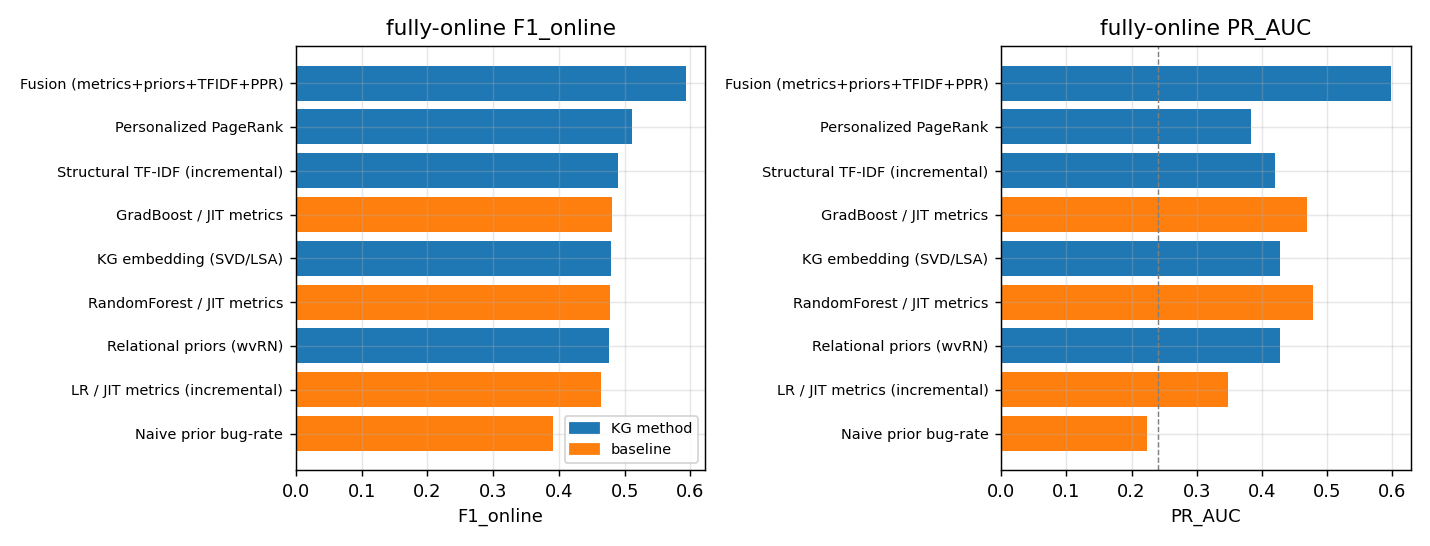
\includegraphics[width=\linewidth]{online_jit_compare.png}\\[3pt]
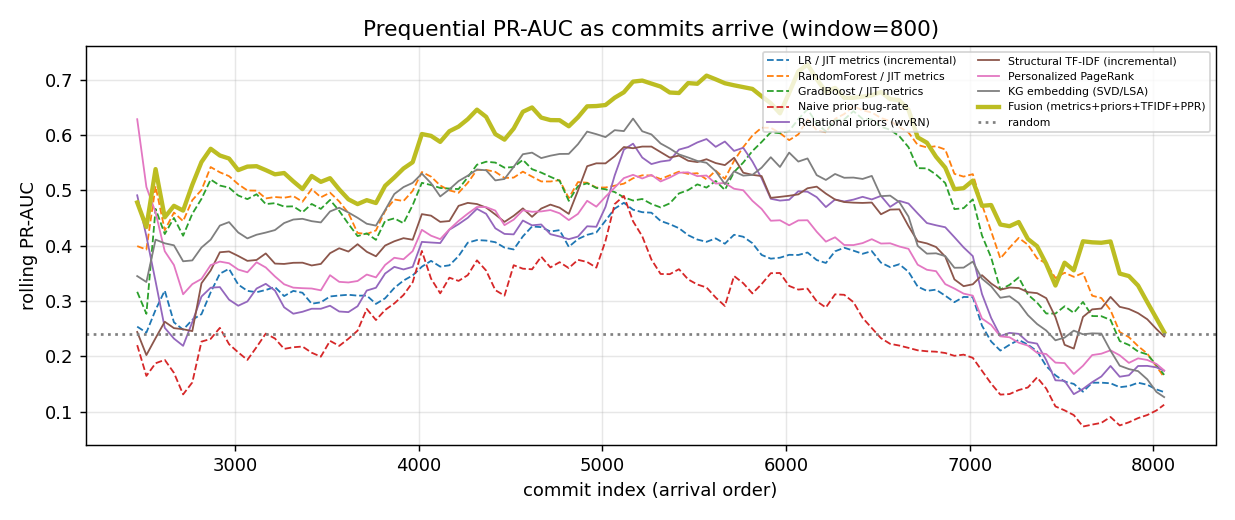
\includegraphics[width=.80\linewidth]{jit_trajectories.png}
\caption{Top: fully-online operating-point F1 (\code{F1\_online}) and PR-AUC
(baselines orange, KG-native blue). Bottom: rolling PR-AUC \emph{as commits
arrive} --- the Fusion (thick blue) stays on top throughout the stream.}\label{fig:jit}
\end{figure}

Under the strict per-commit protocol the \textbf{Fusion again leads on every
metric, including the operating-point F1} (\code{F1\_online} $0.593$ vs.\ $0.481$
for the best baseline), and the trajectory shows the lead is \emph{persistent}.

\paragraph{Fusion feature ablation.} The Fusion combines four streams:
\textbf{M} = JIT metrics, \textbf{T} = structural TF-IDF, \textbf{R} = relational
priors, \textbf{P} = PPR score. We evaluate all $15$ non-empty subsets under the
same online protocol (Figure~\ref{fig:abl}); the leave-one-out drop in
\code{F1\_online} measures each feature's unique contribution.

\begin{figure}[H]\centering
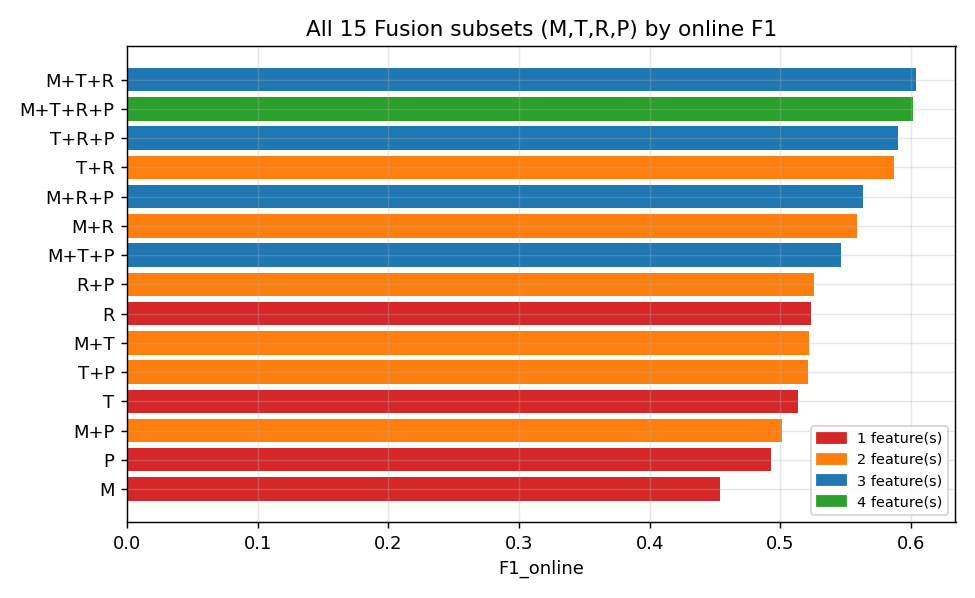
\includegraphics[width=.60\linewidth]{ablation_combos.png}\\[3pt]
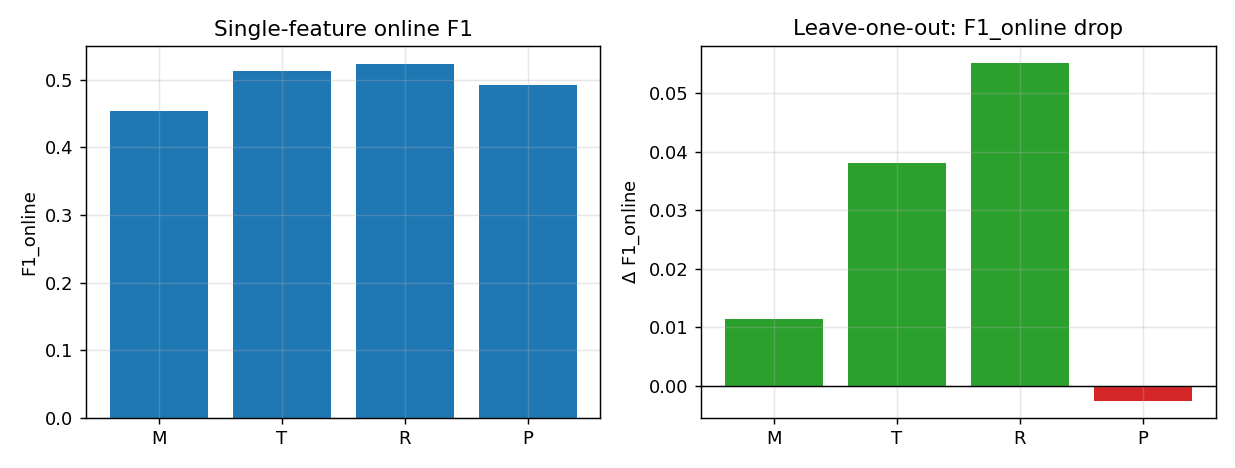
\includegraphics[width=.84\linewidth]{ablation_importance.png}
\caption{Top: all $15$ feature subsets ranked by online F1 (colour $=$ number of
features). Bottom-left: each feature alone. Bottom-right: leave-one-out drop in
\code{F1\_online} when a feature is removed from M+T+R+P (negative $=$ the feature
slightly hurts).}\label{fig:abl}
\end{figure}

Findings (consistent across \code{F1\_online} and PR-AUC):
\begin{itemize}[nosep]
  \item \textbf{Relational priors (R) and structural TF-IDF (T) are the core.}
        They are the strongest single features (\code{F1\_online} $0.52$ / $0.51$)
        and have the largest leave-one-out drops ($-0.055$ and $-0.038$); together
        (T+R) they already reach \code{F1\_online} $0.587$.
  \item \textbf{JIT metrics (M) add a small positive boost}
        (T+R\,$\to$\,M+T+R: $0.587\!\rightarrow\!0.604$).
  \item \textbf{PPR (P) is redundant / marginally harmful}: removing it
        \emph{improves} the result (leave-one-out $+0.003$), so the best subset is
        \textbf{M+T+R} (\code{F1\_online} $0.604$, PR-AUC $0.608$), edging the full
        four-feature fusion --- its graph-proximity signal is already captured by
        the relational priors.
\end{itemize}
\textbf{Recommendation.} The Fusion's sweet spot is \textbf{M+T+R}; PPR can be
dropped with no loss (a small gain) and lower cost.

\paragraph{Reproducibility.} \texttt{python inference/run\_all.py} rebuilds all
features, embeddings (cached under \texttt{outputs/emb\_*.npy}) and the results
cache; the notebook then loads the cache (no Neo4j needed) and draws the
comparison. Per-method entry points: \texttt{train\_eval.py} (tabular ablation),
\texttt{advanced\_infer.py} (TF-IDF/PPR/fusion), \texttt{online\_infer.py}
(prequential O1--O6), \texttt{kge\_infer.py} (node2vec/TransE/DistMult).

% ===========================================================================
\section{Planned Next Steps}\label{sec:next}
% ===========================================================================
\emph{Done in this version:} the finalized online KG build, its audit
(\S\ref{sec:audit}), the online/prequential inference suite of
\S\ref{sec:inference}, and a \emph{controlled} same-split comparison against the
project baselines (\S\ref{sec:cmp}). The controlled comparison reset our
expectations: our fusion is competitive with the tuned traditional-metric
baselines but does \emph{not} yet beat the strong text-based baseline, and our
KG-native methods degrade on the hard low-defect tail window. The next steps,
roughly in priority order, follow directly from that finding.

\begin{enumerate}[nosep]
  \item \textbf{Add commit-message / code text features (highest priority).} The
        single decisive gap in \S\ref{sec:cmp} is that the best baseline uses a
        $768$-dim text embedding while our KG inference uses no text at all.
        Folding message/code text into the fusion (and as \node{Commit}
        properties in the graph) is the most promising near-term gain.
  \item \textbf{Standardise on the controlled evaluation protocol.} Adopt the
        baselines' exact chronological split (train first $70\%$, test last
        $15\%$) as the \emph{common} harness for every method
        (\texttt{inference/compare\_baselines.py}), so all numbers are directly
        comparable. The explicit bar to beat is the text TF-IDF-768D baseline
        (ROC $0.813$ on that split), not merely our own metrics baseline.
  \item \textbf{Graph neural network.} Export per-commit subgraphs (the delta
        plus an $n$-hop AST neighbourhood) and train a GNN --- the model designed
        to exploit the AST structure that the flat/tabular methods discard ---
        evaluated on the controlled protocol above.
  \item \textbf{Robustness across temporal windows.} Investigate why the
        KG-native signals weaken on the low-defect 2018--2019 tail (ROC
        $0.61$--$0.74$ vs.\ much higher on earlier windows): drift-aware
        re-weighting, richer/normalised delta features, and calibration so
        performance holds in sparse-defect regimes.
  \item \textbf{Effort-aware evaluation \& calibration.} Add the JIT-standard
        cost-sensitive metrics ($P_{\text{opt}}$, ACC@20\%LOC) and calibrate the
        relational-prior / wvRN score so its hard-decision (F1) matches its
        already-strong ranking.
  \item \textbf{Bug-localisation supervision.} Connect bug-fixing commits (and,
        via SZZ, the inducing commit) to the AST nodes they repair, creating
        explicit ``defective region'' labels for node-level learning.
  \item \textbf{Richer change semantics.} Distinguish renames from updates;
        optionally fold method-level granularity or data-/control-flow edges into
        the AST layer.
  \item \textbf{Engineering \& scope.} Move the parse-local-id $\rightarrow$
        node-id map onto an \node{ASTNode} property (shrinking the large resumable
        checkpoint) and recover the 6 Java files that fail both parsers. The
        2{,}628 AST-less \texttt{.java} files are full-history files never touched
        by a labelled commit and are \emph{intentionally} out of scope
        (\S\ref{sec:audit}); they would only need ASTs if the labelled study set
        is expanded.
  \item \textbf{Generalisation \& cleanup.} Apply the whole pipeline to other
        ApacheJIT projects to test cross-project transfer; remove the deprecated
        \node{ASTDiff}/\node{ASTEdit} layer.
\end{enumerate}

% ===========================================================================
\section{Legacy Layer}\label{sec:legacy}
% ===========================================================================
An earlier experiment stored each diff as an \node{ASTDiff} summary node with
child \node{ASTEdit} action nodes
(\edge{Commit}$\rightarrow$\edge{HAS\_AST\_DIFF}$\rightarrow$\edge{ASTDiff}$\rightarrow$\edge{EDIT}$\rightarrow$\edge{ASTEdit}).
It is kept for reference (10 diffs, 491 edits) but superseded by the delta layer,
which connects commits to the real AST nodes rather than to standalone summary
nodes, enabling traversal into actual code context.

% ===========================================================================
\appendix
\section{Example Cypher}
% ===========================================================================
\begin{lstlisting}[style=cypher,caption={A commit's delta graph (Graph view).}]
MATCH p = (c:Commit)-[r:ADDS|REMOVES|UPDATES|MOVES]->(a:ASTNode)
WHERE c.id STARTS WITH '6ba7af92'
RETURN p;
\end{lstlisting}

\begin{lstlisting}[style=cypher,caption={Online evaluation window: history known when a commit arrives.}]
MATCH (cur:Commit {id:$id})
MATCH (past:Commit {in_jit:true}) WHERE past.author_ts < cur.author_ts
RETURN count(past) AS known_history,
       sum(CASE WHEN past.buggy THEN 1 ELSE 0 END) AS known_buggy;
\end{lstlisting}

\begin{lstlisting}[style=cypher,caption={Average AST-delta size: buggy vs.\ benign.}]
MATCH (c:Commit {in_jit:true})
OPTIONAL MATCH (c)-[r:ADDS|REMOVES|UPDATES|MOVES]->()
WITH c, count(r) AS delta
RETURN c.buggy AS buggy, count(c) AS commits, round(avg(delta),1) AS avg_delta;
\end{lstlisting}

\paragraph{Visual inspection.} The script
\texttt{viz\_commit\_step.py} produces, for an example commit, the base graph,
the file's AST before the commit, the commit's delta graph, and a single
\emph{overlay} that shows the new nodes/edges (green), removals (red), and
updates (orange) laid on the previous structure --- the recommended way to
visually verify the commit-level modelling.

\end{document}
